\documentclass[a4paper,12pt]{article} % тип документа


% report, book

%  Рисунки
\usepackage{graphicx}
\usepackage{wrapfig}

%  Русский язык

\usepackage[T2A]{fontenc}			% кодировка
\usepackage[utf8]{inputenc}			% кодировка исходного текста
\usepackage[english,russian,]{babel}	% локализация и переносы
\usepackage{xymtex}
\usepackage{amsmath,amsfonts,amssymb,amsthm,mathtools} 
\usepackage{setspace,amsmath}
\usepackage{wasysym}
\usepackage[left=1.27cm,right=1.27cm,top=1.27cm,bottom=2cm, footskip=10mm]{geometry}% настройки полей документа
\RequirePackage{caption2}
\usepackage{float}
\usepackage{ragged2e}
\justifying
%\usepackage[usenames]{color}
\usepackage{icomma} % "Умная" запятая: $0,2$~-— число, $0, 2$~-— перечисление 
\usepackage{upgreek} 
%\usepackage[14pt]{extsizes} % для того чтобы задать нестандартный 14-ый размер шрифта

\usepackage{gensymb}
\usepackage{esint}
\usepackage{gnuplottex} 

%%% Оформление 
\usepackage{indentfirst} % Красная строка 
\setlength{\parskip}{0.3cm} % отступы между абзацами 

%%% Теоремы 
\theoremstyle{plain} % Это стиль по умолчанию, его можно не переопределять. 
\newtheorem{theorem}{Теорема}[section] 
\newtheorem{proposition}[theorem]{Утверждение} 

\theoremstyle{definition} % "Определение" 
\newtheorem{definition}{Определение}[section] 
\newtheorem{corollary}{Следствие}[theorem] 
\newtheorem{problem}{Задача}[section] 

\theoremstyle{remark} % "Примечание" 
\newtheorem*{nonum}{Решение} 
\newtheorem{zamech}{Замечание}[theorem] 



% новая команда \RNumb для вывода римских цифр
\newcommand{\RNumb}[1]{\uppercase\expandafter{\romannumeral #1\relax}}

\begin{document} % начало документа
 
% НАЧАЛО ТИТУЛЬНОГО ЛИСТА
\begin{center}
\hfill \break
{МИНИСТЕРСТВО НАУКИ И ВЫСШЕГО ОБРАЗОВАНИЯ РОССИИ}\\
\footnotesize{ФЕДЕРАЛЬНОЕ ГОСУДАРСТВЕННОЕ АВТОНОМНОЕ ОБРАЗОВАТЕЛЬНОЕ}\\ 
\footnotesize{УЧРЕЖДЕНИЕ ВЫСШЕГО ОБРАЗОВАНИЯ}\\
\small{\textbf{«МОСКОВСКИЙ ФИЗИКО-ТЕХНИЧЕСКИЙ ИНСТИТУТ (НАЦИОНАЛЬНЫЙ ИССЛЕДОВАТЕЛЬСКИЙ УНИВЕРСИТЕТ)»}}\\
\hfill \break
\normalsize{Факультет биологической и медицинской физики}\\
\hfill \break

\hfill \break
\hfill \break
\hfill \break
\hfill\break
\hfill\break
\large\textbf{{Лабораторная работа 2.5.1}}\\
\large{Измерение коэффициента поверхностного натяжения жидкости}\\
\hfill \break
\hfill \break
\end{center}
 
\begin{flushright}
{Выполнили:}

{Синькин Александр Вадимович,\\ Кузь Глеб Сергеевич}

{группа Б06-801}
\end{flushright}

\hfill \break
\begin{center} Долгопрудный,  \today \end{center}
\thispagestyle{empty} % выключаем отображение номера для этой страницы
 
% КОНЕЦ ТИТУЛЬНОГО ЛИСТА

\newpage

\section*{Измерение коэффициента поверхностного натяжения жидкости.}

\textbf{Цель работы:} \textit{1) измерение температурной зависимости  коэффициента поверхностного натяжения дистиллированной воды с использованием известного коэффициента поверхностного натяжения спирта;  2) определение полной поверхностной энергии  и теплоты, необходимой для изотермического образования единицы  поверхности жидкости  при различной температуре. }

\textbf{В работе используются:} \textit{ прибор  Ребиндера  с термостатом и микроманометром; исследуемые жидкости; стаканы.}


Наличие поверхностного слоя приводит к различию давлений по разные стороны от искривленной границы раздела двух сред.  Для сферического пузырька с воздухом  внутри жидкости избыточное давление даётся формулой Лапласа:
\begin{equation}
P = P_{\text{внутри}} - P_{\text{снаружи}} =  \dfrac{2\sigma }{r} ,
\end{equation}
где $\sigma$ – коэффициент поверхностного натяжения, $P_{\text{внутри}}$ и $P_{\text{снаружи}}$ – давление внутри пузырька и снаружи, $r$ – радиус кривизны поверхности раздела двух фаз. Эта формула лежит в основе предлагаемого метода определения коэффициента поверхностного натяжения жидкости. Измеряется давление $\Delta P$, необходимое для выталкивания в жидкость пузырька воздуха.

\textbf{Экспериментальная установка.} Исследуемая жидкость (дистиллированная вода) наливается в сосуд (колбу) В (рис.1). Тестовая жидкость  (этиловый спирт) наливается  в сосуд Е.  При измерениях  колбы герметично закрываются  пробками.   Через одну из двух пробок  проходит полая металлическая игла С. Этой пробкой закрывается сосуд, в котором  проводятся измерения. Верхний конец иглы открыт в атмосферу, а нижний погружен в жидкость. Другой сосуд герметично закрывается второй пробкой. При создании достаточного  разряжения воздуха в колбе с иглой пузырьки воздуха начинают пробулькивать через жидкость. Поверхностное натяжение можно определить по величине разряжения $\Delta P$ (1), необходимого для прохождения пузырьков (при известном радиусе иглы).

\begin{figure}[H]
	\begin{center}
	 	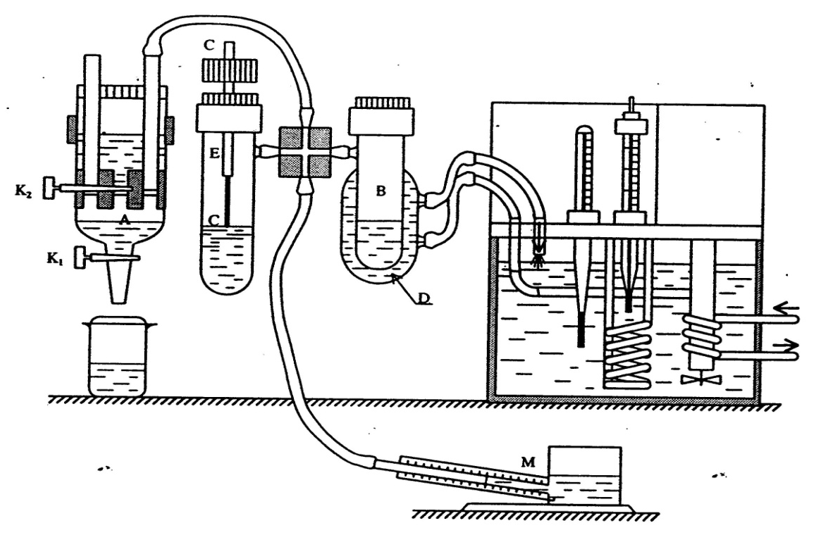
\includegraphics[scale=0.8]{Pic_1}
 		\caption{Схема установки для измерения температурной зависимости коэффициента поверхностного натяжения}
	\end{center}
\end{figure}

Разряжение в системе создается с помощью аспиратора А. Кран $K_2$ разделяет две полости аспиратора. Верхняя полость при закрытом кране К2  заполняется водой. Затем кран $K_2$ открывают и заполняют водой  нижнюю полость  аспиратора.  Разряжение воздуха создается в нижней полости  при открывании крана $K_1$, когда  вода вытекает из неё по каплям. В колбах В и С, соединённых трубками с нижней полостью аспиратора,  создается такое же пониженное давление. Разность давлений в полостях с разряженным воздухом и атмосферой измеряется спиртовым микроманометром (устройство микроманометра описано в Приложении). 

Для стабилизации температуры исследуемой жидкости через рубашку D колбы В непрерывно прогоняется вода из термостата.

Обычно кончик иглы лишь касается поверхности жидкости, чтобы исключить влияние гидростатического давления столба жидкости. Однако при измерении температурной зависимости коэффициента поверхностного натяжения возникает ряд сложностей. Во-первых, большая теплопроводность металлической трубки приводит к тому, что температура на конце трубки заметно ниже, чем в глубине жидкости. Во-вторых, тепловое расширение поднимает уровень жидкости при увеличении температуры. 

Обе погрешности можно устранить, погрузив кончик трубки до самого дна. Полное давление, измеренное при этом микроманометром, $P = \Delta P + \rho gh$. Заметим, что $\rho gh$ от температуры практически не зависит, так как подъём уровня жидкости компенсируется уменьшением её плотности (произведение $\rho h$ определяется массой всей жидкости и поэтому постоянно). Величину  $\rho gh$ следует измерить двумя способами. Во-первых, замерить величину $P_1= \Delta P'$, когда кончик трубки только касается поверхности жидкости. Затем при этой же температуре опустить иглу до дна и замерить $P_2= \rho gh + \Delta P''$ ($\Delta P', \Delta P''$ – давление Лапласа). Из-за  несжимаемости  жидкости можно положить $\Delta P' = \Delta P''$ и тогда $\rho gh = P_2-P_1.$ Во-вторых, при измерениях $P_1$ и $P_2$ замерить линейкой  глубину погружения иглы $h$. Это можно сделать, замеряя расстояние между верхним концом иглы и любой неподвижной частью прибора при положении иглы на поверхности и в глубине колбы.

\textbf{Замечание.} Чувствительность микроманометра высока, поэтому правильность его работы существенно зависит от правильности  эксплуатации прибора. \textbf{Все изменения в установке необходимо проводить, предварительно поставив переключатель микроманометра на атмосферу.}

В частности подобную же операцию необходимо сделать и при заполнении водой аспиратора А. В противном случае при заполнении аспиратора водой давление воздуха в системе повышается, спирт из трубки микроманометра выдавливается, в узлах соединений микроманометра образуются воздушные пузыри. Наличие этих пузырей приводит к полному нарушению калибровки манометра и невоспроизводимости измерений.

\newpage

\begin{center}
\section*{ЗАДАНИЕ.}
\end{center}

1. Проверьте герметичность установки. Для этого заполните аспиратор водой. Чистую сухую иглу установите в сосуд со спиртом так, чтобы кончик иглы лишь касался поверхности спирта. Плотно закройте обе колбы В и Е пробками. Откройте кран $K_1$ аспиратора и добейтесь пробулькивания пузырьков воздуха в колбе. Замерьте показания микроманометра. Закройте кран $K_1$. Наблюдайте за показаниями манометра: при отсутствии течи в установке столбик спирта в манометре будет неподвижен. При наличии течи следует обратиться к преподавателю или лаборанту.

2. Убедившись в герметичности системы, начните измерения. Откройте кран $K_1$. Подберите частоту падения капель из аспиратора так, чтобы максимальное давление манометра не зависело от этой частоты (не чаще, чем 1 капля в 5 секунд).

3. Измерьте максимальное давление $\Delta P_{\text{спирт}}$  при  пробулькивании пузырьков воздуха через спирт. По разбросу результатов оцените случайную погрешность измерения. Пользуясь табличным значением коэффициента поверхностного натяжения спирта, определите по формуле (1) диаметр иглы. Сравните полученный результат с диаметром иглы, измеренным по микроскопу.

4. Перенесите предварительно промытую и просушенную от спирта иглу в колбу с дистиллированной водой. Измерьте максимальное давление $P_1$ при пробулькивании пузырьков, когда игла лишь касается поверхности воды. Аспиратор должен быть предварительно  заполнен водой почти доверху. Отрегулируйте скорость поднятия уровня спирта в манометре и сохраняйте её в течение всех экспериментов. Измерьте расстояние между верхним концом иглы и любой неподвижной часть прибора $h_1$.

5. Утопите иглу до предела (между концом иглы и дном необходимо оставить небольшой зазор, чтобы образующийся пузырёк не касался дна). Измерьте $h_2$ (как в пункте 4).

Измерьте максимальное давление в пузырьках $P_2$. По разности давлений $\Delta P = P_2 - P_1$ определите глубину погружения $\Delta h$ иглы и сравните с $\Delta h =  h_1- h_2.$ 

6. Снимите температурную зависимость $\sigma(T)$ дистиллированной воды. Для этого включите термостат и подождите, пока нужная вам температура не стабилизируется. Следует заметить, что термометр показывает температуру воды в термостате. Время установления заданной температуры в колбе с исследуемой жидкостью довольно большое, поэтому после установления заданной температуры в термостате дождитесь прогрева исследуемой жидкости в колбе в течение нескольких минут (5-7 минут). После этого проведите измерение давления. Для уменьшения погрешности опыта замер давления  при фиксированной температуре следует проводить несколько раз. 
Проводить измерение температурной зависимости  рекомендуется в диапазоне  $\rm 20^{\circ}C - 60^{\circ}C$ через $\rm 5^{\circ}C$. Запрещается нагревать воду в термостате выше $\rm 60^{\circ}C$.

7. Оцените погрешность измерения давления и температуры. Рассчитайте величину коэффициента поверхностного натяжения воды $\sigma (T)$, используя значение диаметра иглы, полученное при измерениях на спирте (или измеренное на микроскопе).

8. Постройте график зависимости $\sigma (T)$ и определите по графику температурный коэффициент  $\dfrac{d\sigma}{dT}$. Оцените точность результата.

9. На другом графике постройте зависимость от температуры

а) теплоты образования единицы поверхности жидкости $q=\ -T\cdot \dfrac{d\sigma}{dT}$   и 

б) поверхностной энергии $U$ единицы площади $F$:  $\dfrac{U}{F} = (\sigma -T\cdot \dfrac{d\sigma}{dT} ).$ 




\end{document}